\documentclass{article}

%change the margin of the paper
%\usepackage[legalpaper, margin=0.1in]{geometry}
%using the \substack
\usepackage{amsmath}
% \mathbbm{}
\usepackage{bbm}

% hyperlink Here
\usepackage{hyperref}
\hypersetup{
    colorlinks=true,
    linkcolor=blue,
    filecolor=magenta,
    urlcolor=cyan,
}

% this is the package for block comment \begin{comment} and \end{comment}
\usepackage{verbatim}
\usepackage{imakeidx}
% For multiple rows in tabular environment.
\usepackage{multirow}
% use this package to strikeout the word /st{}
%the color package is for the \textcolor{red} to highlight the text
\usepackage{color,soul}
% to define newcolumntype and \arraybackslash
\usepackage{array}
% hyperref is to call /url. hyphen packege to avoid that the url is too long
\PassOptionsToPackage{hyphens}{url}\usepackage{hyperref}
%Todo list, \newlist \setlist...
\usepackage{enumitem,amssymb}
\newlist{todolist}{itemize}{2}
\setlist[todolist]{label=$\square$}

% for image inserting
\usepackage{graphicx}
\graphicspath{./Desktop/Homework/123/6/}
\usepackage{subfig}

% \iff \leqlsant
\usepackage{amssymb}



% Code block begin(lstlisting) and end(lstlisting)
\usepackage{listings}
\usepackage{color}

\definecolor{dkgreen}{rgb}{0,0.6,0}
\definecolor{gray}{rgb}{0.5,0.5,0.5}
\definecolor{mauve}{rgb}{0.58,0,0.82}


%NOTE: Change the "language" parameter here
\lstset{frame=tb,
  language=Matlab,
  aboveskip=3mm,
  belowskip=3mm,
  showstringspaces=false,
  columns=flexible,
  basicstyle={\small\ttfamily},
  numbers=none,
  numberstyle=\tiny\color{gray},
  keywordstyle=\color{blue},
  commentstyle=\color{dkgreen},
  stringstyle=\color{mauve},
  breaklines=true,
  breakatwhitespace=true,
  tabsize=3
}

% Macros
%%%%%%%%%%%% Text Color %%%%%%%%%%%%%%%
\definecolor{mypink1}{RGB}{219, 48, 233}
\definecolor{myred1}{RGB}{231, 76, 60}
\definecolor{myred2}{RGB}{203, 67, 53}
\definecolor{myblue1}{RGB}{52, 152, 219}
\definecolor{mygray}{gray}{0.6}

%% Table Style
\newcolumntype{C}{>{\center\arraybackslash}m{.70\columnwidth}}
\newcolumntype{Y}{>{\center\arraybackslash}m{2cm}}




%NOTE title Here
\title{Math 123 Homework 6}
\author{Hanyuan Zhu}


\begin{document}

\maketitle

\subsection*{Question 1}

\paragraph{(a)}

\begin{equation}
  vol(C) = \sum_{\substack{x_{i} \in C \\ x_{j} \in V}} W_{ij} = \sum_{\substack{x_{i} \in C \\ x_{j} \in N(x_{i})}} W_{ij}
\end{equation}
$N(x_{i})$ is the set of neighorhood of $x_i$, $(x_{j}|w_{ij} \neq 0, for \quad x_{i})$


\begin{equation}
  D_{ii} = \sum_{x_j \in N(x_{i})} W_{ij}
\end{equation}

\begin{equation}
  (Df^{C})_{i} = \begin{cases} -\sum_{x_j \in N(x_{i})} W_{ij} \sqrt{vol(\bar{C})/vol{C})} & x_{i} \in C\\
                                \sum_{x_j \in N(x_{i})} W_{ij} \sqrt{vol(C)/vol{\bar{C}})} & x_{i} \in \bar{C}
                  \end{cases}
\end{equation}


\begin{equation}
  \begin{split}
  \langle Df^{C} \cdot  \mathbbm{1} \rangle & =  \sum_{x_i \in V} (Df^{C})_{i} = \sum_{x_i \in C} (Df^{C})_{i} +\sum_{x_i \in \bar{C}} (Df^{C})_{i} \\
  & \overset{(3)}{=} -\sum_{\substack{x_{i} \in C \\ x_{j} \in V}} W_{ij} \sqrt{vol(\bar{C})/vol(C)} + \sum_{\substack{x_{i} \in \bar{C} \\ x_{j} \in V}} W_{ij} \sqrt{vol(C)/vol(\bar{C})}\\
  & = - \sqrt{vol(\bar{C})/vol(C)} \cdot \sum_{\substack{x_{i} \in C \\ x_{j} \in V}} W_{ij}  + \sqrt{vol(C)/vol(\bar{C})} \cdot \sum_{\substack{x_{i} \in \bar{C} \\ x_{j} \in V}} W_{ij} \\
  & \overset{(1)}{=} - \sqrt{vol(\bar{C})/vol(C)} \cdot vol(C) + \sqrt{vol(C)/vol(\bar{C})} \cdot vol(\bar{C})\\
  & = - \sqrt{vol(\bar{C})vol(C)} +\sqrt{vol(C) vol(\bar{C})} \\
  & = 0
  \end{split}
\end{equation}

\paragraph{(b)}

\begin{equation}
  \begin{split}
    (f^C)^T Df^{C} & = \sum_{x_i \in V} f^{C}(x_i) (\sum_{x_j \in N(x_i)} W_{ij}) f^{C}(x_i)\\
    & = \sum_{x_i \in V} (f^{C}(x_i))^2 (\sum_{x_j \in N(x_i)} W_{ij})\\
    & = \sum_{x_i \in C} (f^{C}(x_i))^2 (\sum_{x_j \in N(x_i)} W_{ij}) +  \sum_{x_i \in \bar{C}} (f^{C}(x_i))^2 (\sum_{x_j \in N(x_i)} W_{ij})\\
    & = vol(C) \frac{vol(\bar{C})}{vol(C)}  + vol(\bar{C})\frac{vol(C)}{vol(\bar{C})} \\
    & = vol(\bar{C}) + vol(C)\\
    & = \sum_{\substack{x_{i} \in \bar{C} \\ x_{j} \in V}} W_{ij} +\sum_{\substack{x_{i} \in C \\ x_{j} \in V}} W_{ij} = \sum_{\substack{x_{i} \in V \\ x_{j} \in V}} W_{ij} \\
    & = vol(V)
\end{split}
\end{equation}

\paragraph{(c)}
\begin{equation}
  \begin{split}
    (f^C)^T Lf^{C} & = (f^C)^T (D-W) f^{C} = (f^C)^T Df^{C} - (f^C)^T Wf^{C}
  \end{split}
\end{equation}
We know that
\begin{equation}
  (f^C)^T Df^{C} = vol(V)
\end{equation}


And
\begin{equation}
  \begin{split}
  (f^C)^T Wf^{C} & = \sum_{\substack{x_{i} \in V \\ x_{j} \in V}} W_{ij} f^{C}_i f^{C}_j  \\
  & = \sum_{\substack{x_{i} \in C \\ x_{j} \in C}} W_{ij} f^{C}_i f^{C}_j + \sum_{\substack{x_{i} \in \bar{C} \\ x_{j} \in \bar{C}}} W_{ij} f^{C}_i f^{C}_j + \sum_{\substack{x_{i} \in C \\ x_{j} \in \bar{C}}} W_{ij} f^{C}_i f^{C}_j + \sum_{\substack{x_{i} \in \bar{C} \\ x_{j} \in C}} W_{ij} f^{C}_i f^{C}_j
  \end{split}
\end{equation}

Notice that\[
f^{C}_i f^{C}_j = \begin{cases} \frac{vol(\bar{C})}{vol(C)} & x_{i} \in C and x_{j} \in C \\
\frac{vol(C)}{vol(\bar{C})}, & x_{i} \in \bar{C} and x_{j} \in \bar{C}\\
-1 &  x_{i} \in \bar{C} and x_{j} \in C, or x_{i} \in C and x_{j} \in \bar{C}
\end{cases}
\], and we define $\sum_{\substack{x_i \in C \\ x_j \in \bar{C}}} W_{ij} = \sum_{\substack{x_i \in \bar{C} \\ x_j \in C}} W_{ij} =: \frac{1}{2}vol(B)$.

Then (8) turns out to be
\begin{equation}
  \begin{split}
  (8) & = \sum_{\substack{x_{i} \in C \\ x_{j} \in C}} W_{ij} \frac{vol(\bar{C})}{vol(C)}  + \sum_{\substack{x_{i} \in \bar{C} \\ x_{j} \in \bar{C}}} W_{ij} \frac{vol(C)}{vol(\bar{C})} - \sum_{\substack{x_{i} \in C \\ x_{j} \in \bar{C}}} W_{ij} - \sum_{\substack{x_{i} \in \bar{C} \\ x_{j} \in C}} W_{ij} \\
  & = \frac{vol(\bar{C})}{vol(C)} \sum_{\substack{x_{i} \in C \\ x_{j} \in C}} W_{ij} +  \frac{vol(C)}{vol(\bar{C})} \sum_{\substack{x_{i} \in \bar{C} \\ x_{j} \in \bar{C}}} W_{ij} - \frac{1}{2}vol(B) - \frac{1}{2}vol(B)\\
  & =  \frac{vol(\bar{C})}{vol(C)}(\sum_{\substack{x_{i} \in C \\ x_{j} \in V}}W_{ij} -\sum_{\substack{x_{i} \in C \\ x_{j} \in \bar{C}}}W_{ij})  +\frac{vol(C)}{vol(\bar{C})} (\sum_{\substack{x_{i} \in \bar{C} \\ x_{j} \in V}} W_{ij}- \sum_{\substack{x_{i} \in \bar{C} \\ x_{j} \in C}}W_{ij}) - vol(B)\\
  & =  \frac{vol(\bar{C})}{vol(C)}(vol(C)-\frac{1}{2}vol(B)) + \frac{vol(C)}{vol(\bar{C})}(vol(\bar{C})-\frac{1}{2}vol(B)) - vol(B)\\
  & = vol(\bar{C}) - \frac{1}{2}vol(B))\frac{vol(\bar{C})}{vol(C)} + vol(C) - \frac{1}{2}vol(B)\frac{vol(C)}{vol(\bar{C})} - vol(B)\\
  & = vol(V) - \frac{1}{2} vol(B)(\frac{vol(\bar{C})}{vol(C)}+\frac{vol(C)}{vol(\bar{C})}+2)\\
  & = vol(V) -  \frac{1}{2} vol(B)(\sqrt{\frac{vol(\bar{C})}{vol(C)}} + \sqrt{\frac{vol(C)}{vol(\bar{C})}})^2\\
  & = vol(V) -  \frac{1}{2}vol(B)\frac{(\sqrt{vol(\bar{C})}\sqrt{vol(\bar{C})}+\sqrt{vol(C)} \sqrt{vol(C)})^2}{vol(\bar{C})vol(C)}\\
  & = vol(V) -  \frac{1}{2}vol(B)\frac{vol(V)^2}{vol(\bar{C})vol(C)}\\
  & = vol(V) -  \frac{1}{2}vol(B)vol(V)\frac{vol(V)}{vol(\bar{C})vol(C)}\\
  & = vol(V) -  \frac{1}{2}vol(B)vol(V)\frac{vol(\bar{C})+vol(C)}{vol(\bar{C})vol(C)}\\
  & = vol(V) -  \frac{1}{2}vol(B)vol(V)(\frac{1}{vol(\bar{C})}+\frac{1}{vol(C)})\\
  & = vol(V) - vol(V) Ncut(C,\bar{C})
\end{split}
\end{equation}
, where $Ncut(C,\bar{C}) = \sum_{\substack{x_i \in C \\ x_j \in \bar{C}}} W_{ij} (\frac{1}{vol(\bar{C})}+\frac{1}{vol(C)}) = \frac{1}{2}vol(B)(\frac{1}{vol(\bar{C})}+\frac{1}{vol(C)})$

Substitute (7) and (9) into (6), we have
\begin{equation}
  \begin{split}
  (f^C)^T Lf^{C} & = (f^C)^T (D-W) f^{C} = (f^C)^T Df^{C} - (f^C)^T Wf^{C}\\
  & = vol(V) - (vol(V) - vol(V) Ncut(C,\bar{C}))\\
  & = vol(V) Ncut(C,\bar{C})
\end{split}
\end{equation}

\subsection*{Question 2}
\paragraph{(a)}

Because  $$ L_{ij} = \begin{cases} -W_{ij} & i \neq j\\ \sum_{\substack{x_j \in V \\ i \neq j}} W_{ij} & i = j \end{cases}$$,
and $$\lim_{\sigma \rightarrow 0} W_{ij} = \lim_{\sigma \rightarrow 0} e^{-\frac{||x_{i}-x_{j}||_{2}^{2}}{\sigma^{2}}} = 0 $$,
then $$ \lim_{\sigma \rightarrow 0} L_{ij} = 0 $$.

Therefore, all eigenvalues are 0s and any $v \in \mathbb{R}^n/{\vec{0}}$ are the eighenvectors.

\paragraph{(b)}
Since $$\lim_{\sigma \rightarrow \infty} W_{ij} = \lim_{\sigma \rightarrow \infty} e^{-\frac{||x_{i}-x_{j}||_{2}^{2}}{\sigma^{2}}} = 1 $$,
then $$ \lim_{\sigma \rightarrow \infty} L_{ij} = \begin{cases} -1, & i \neq j \\ n-1, & i=j  \end{cases} $$

It is equivalent to a unweighted complete graph. Therefore, it has one egenvalue at 0, and other eigenvalues at n. The eigenvector of 0 is $\mathbbm{1}$ and all other eigenvector are distinct.

\subsection*{Question 3}
\paragraph{(a)}
We choose sigma = 50000 here and k =6. When the knn is about 15 to 25, the clusters looks similar to grountruth.

Firstly, it is clear that our result shows less infomation than grountruth, because the groundtruth has 14 categories, while we only have 6 clusters (in eigenspace) for kmean method.

Secondly, When knn is too small, the weighted degree of different nodes various too much. Some points in " very dense" area become outliers in eighenspace, which results in kmean producing poor clusters( lots of clusters are outliers only).
\begin{figure}
  \centering
  \subfloat[ knn=5 ]{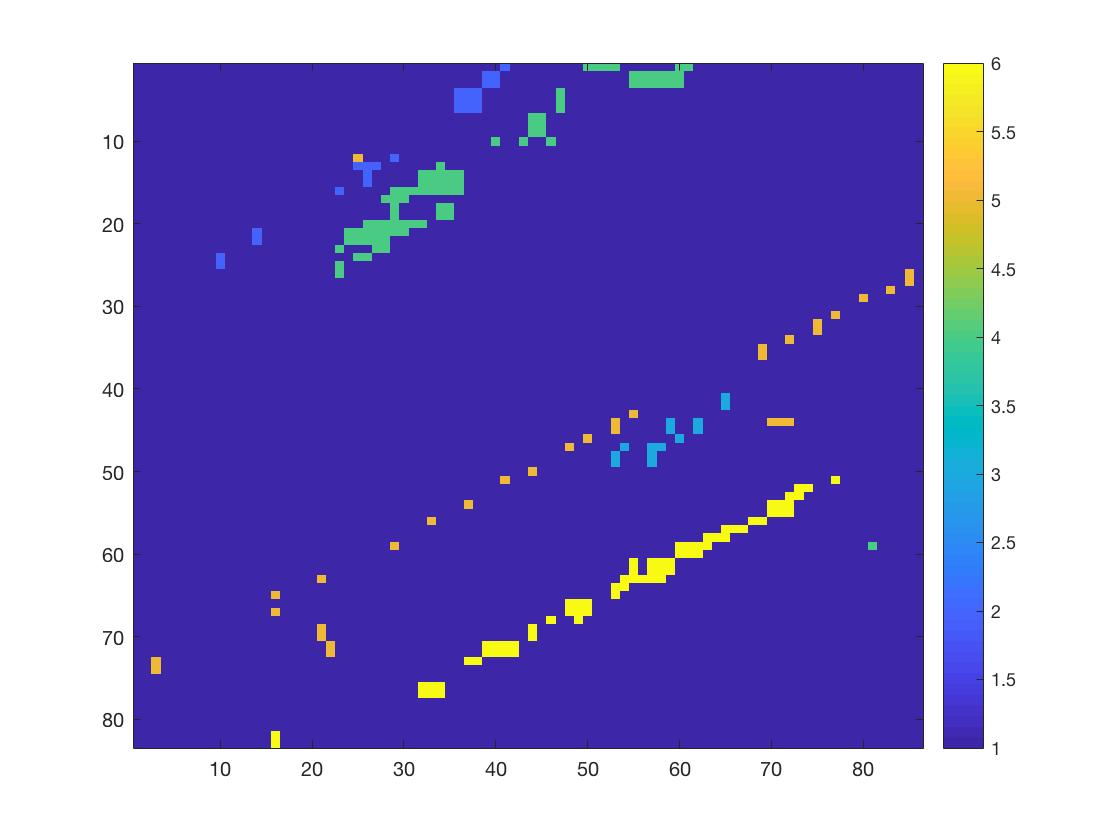
\includegraphics[width=4cm, height=4cm]{pic/sigma50000knn5.jpg}}
  \qquad
  \subfloat[ knn=15 ]{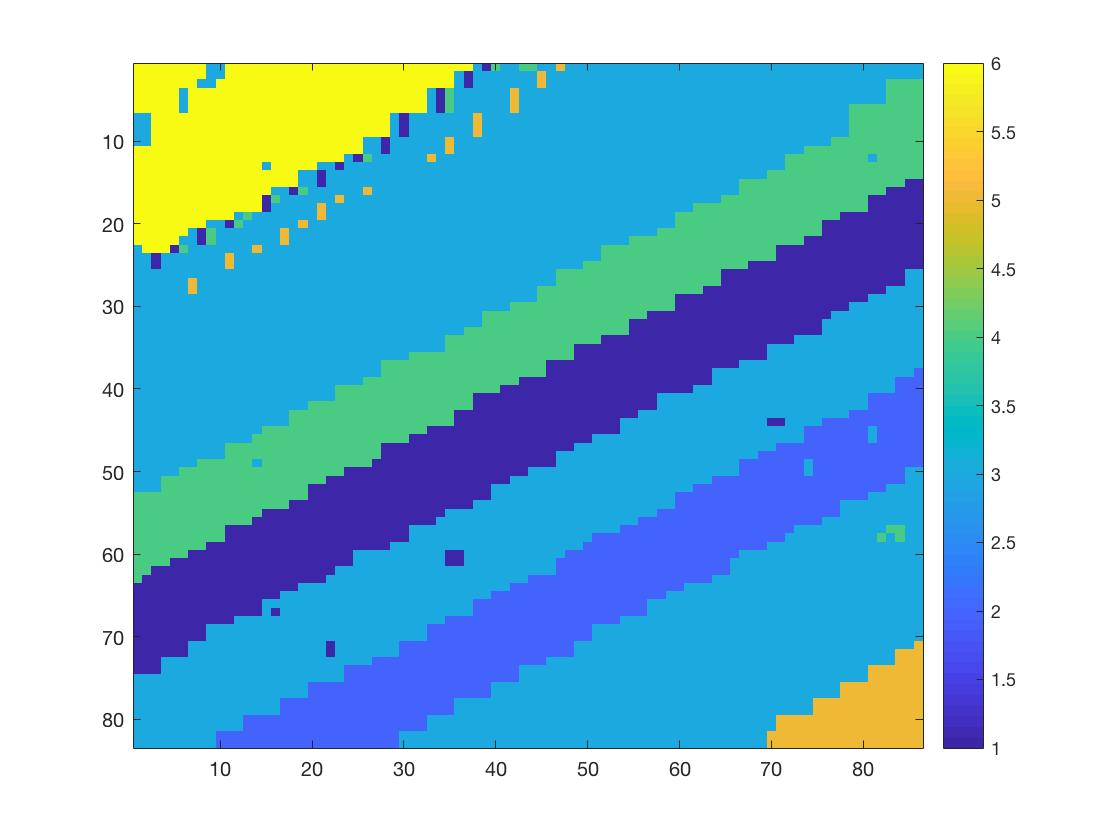
\includegraphics[width=4cm, height=4cm]{pic/sigma50000knn15}}
\end{figure}
\begin{figure}
  \centering
  \subfloat[ knn=25 ]{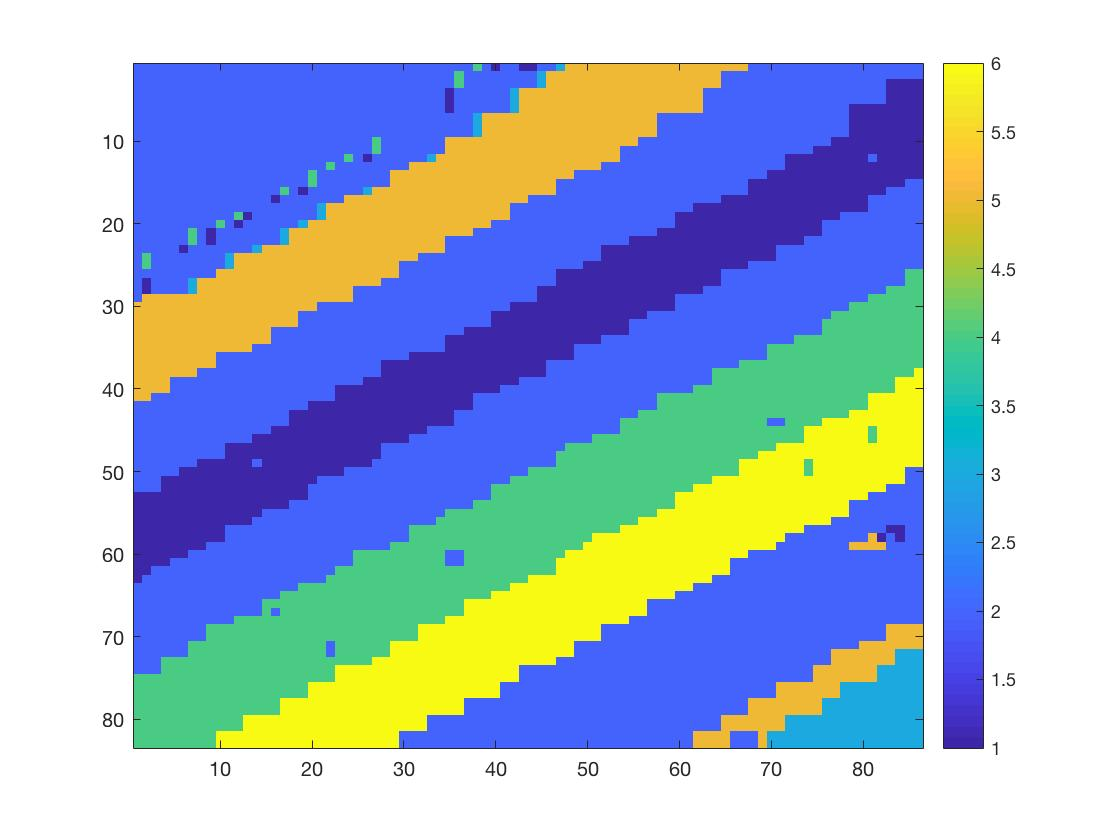
\includegraphics[width=4cm, height=4cm]{pic/sigma50000knn25}}
  \qquad
  \subfloat[ knn=50 ]{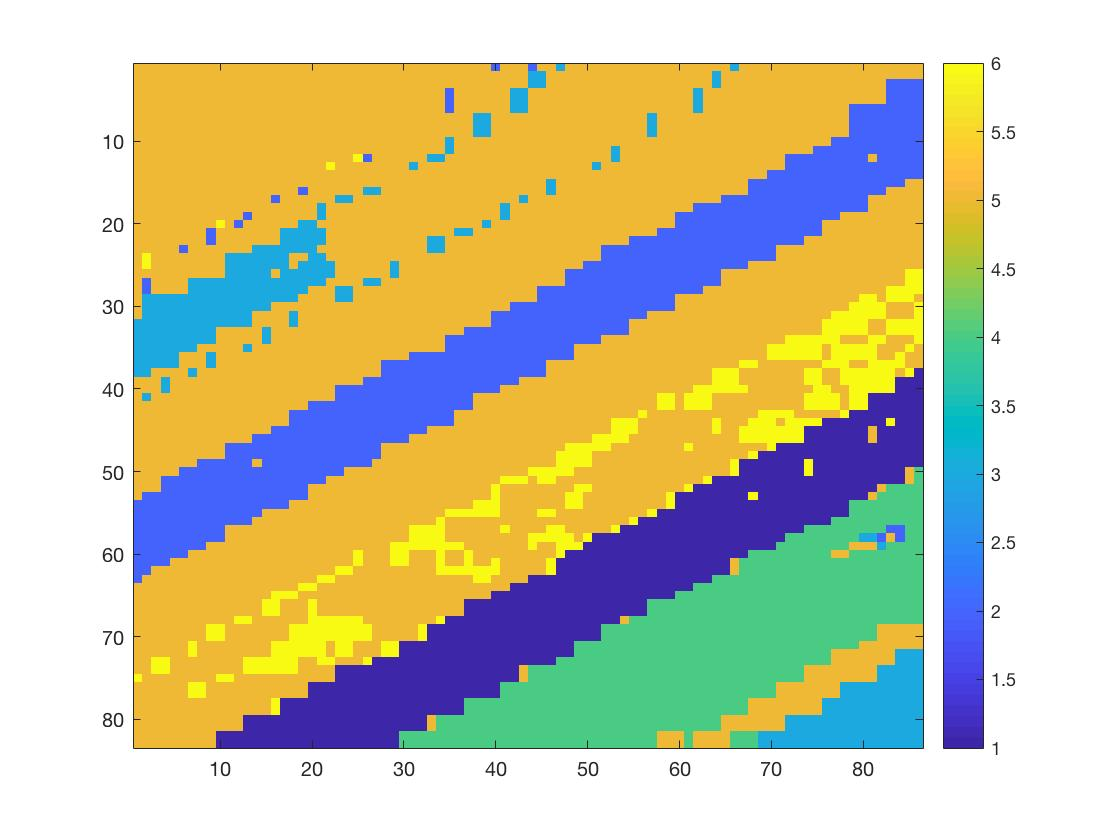
\includegraphics[width=4cm, height=4cm]{pic/sigma50000knn50}}
  \qquad
  \subfloat[ groundtruth ]{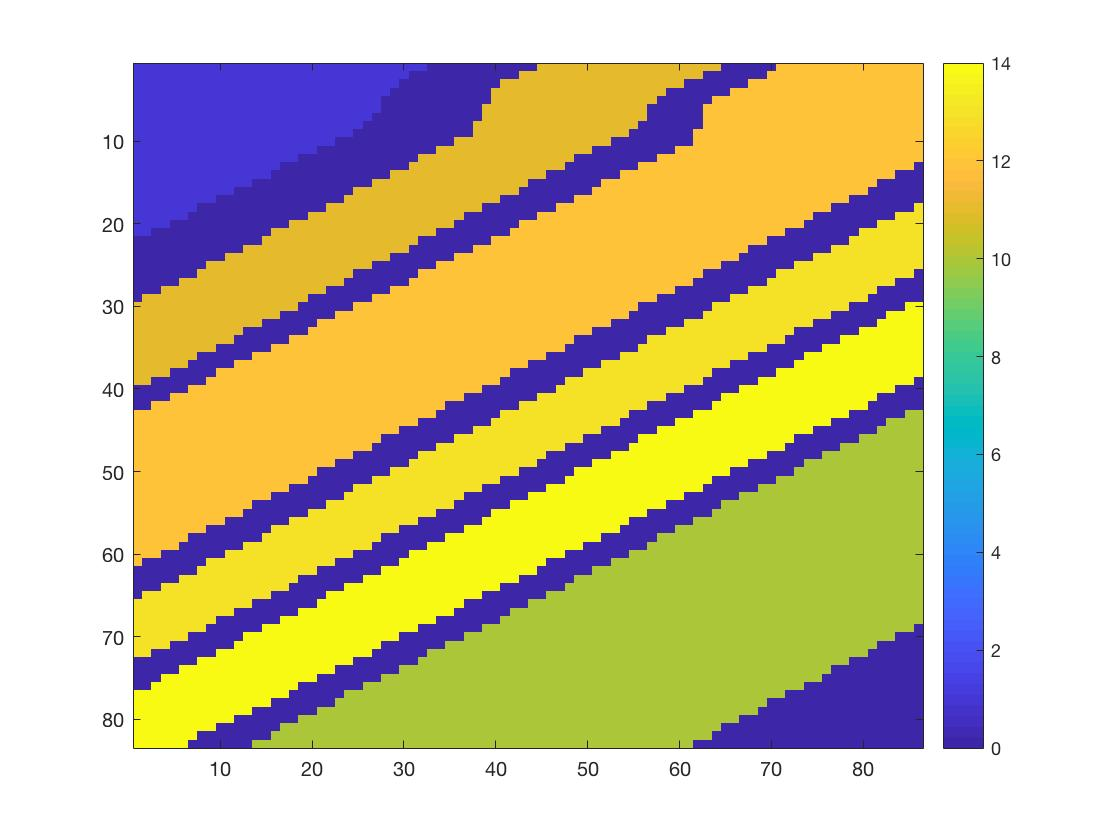
\includegraphics[width=4cm, height=4cm]{pic/groundtruth}}
\end{figure}



\newpage
\paragraph{(b)}
As $\sigma$ increase, the eigengaps increase about same order as $\sigma$ does.
\begin{figure}
  \centering
  \subfloat[ sigma=500 ]{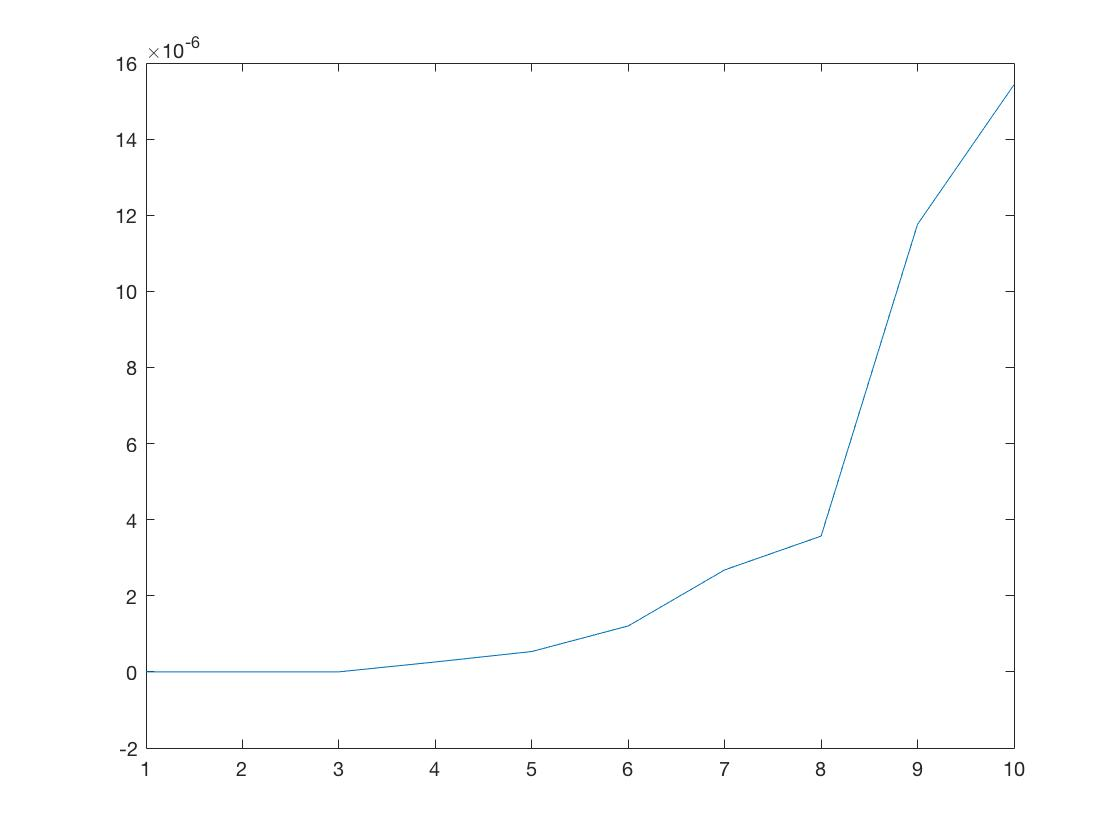
\includegraphics[width=4cm, height=4cm]{pic/vs500}}
  \qquad
  \subfloat[ sigma=5000 ]{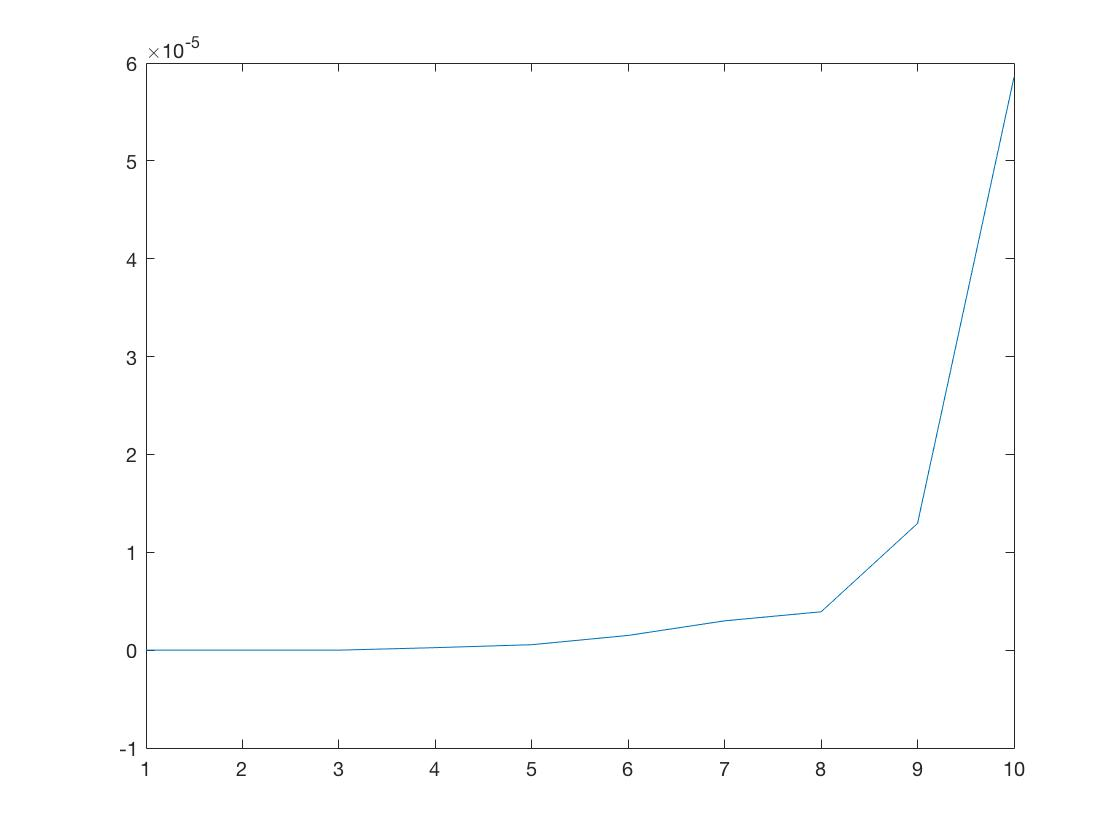
\includegraphics[width=4cm, height=4cm]{pic/vs5000}}
  \qquad
  \subfloat[ sigma=50000 ]{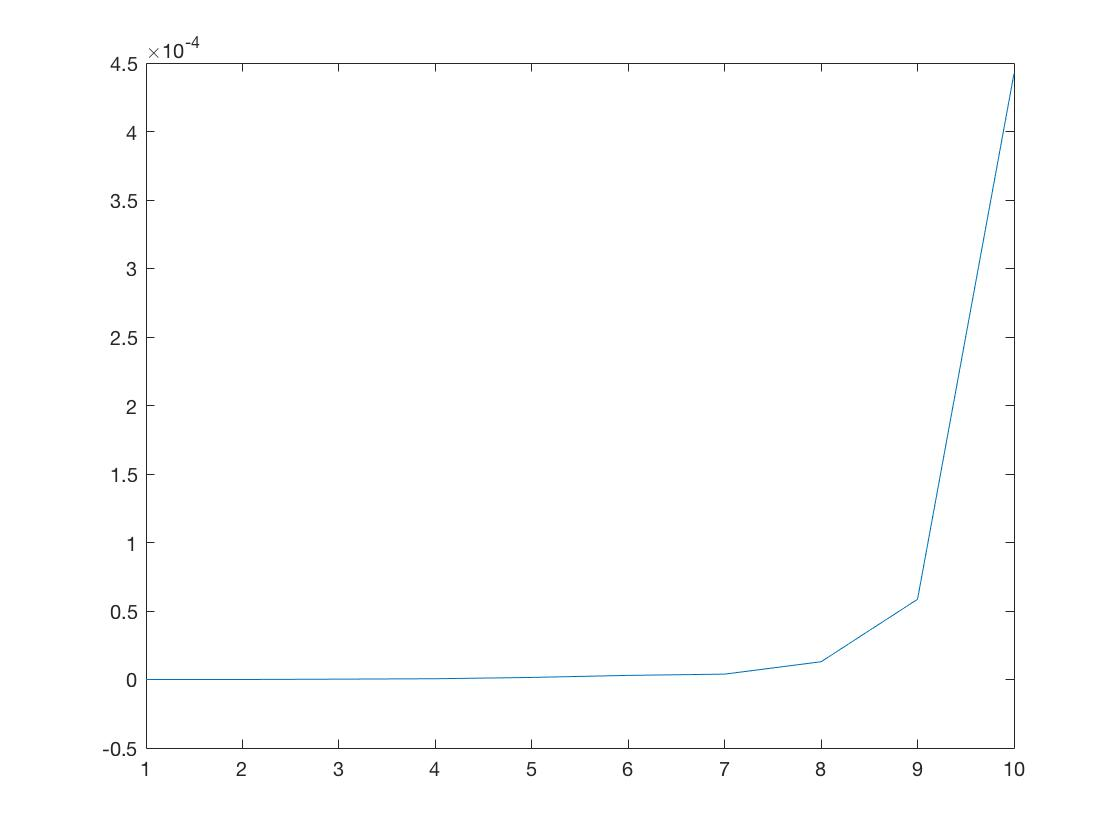
\includegraphics[width=4cm, height=4cm]{pic/vs50000}}
\end{figure}


\paragraph{(c)}
The PCA plot represent a frequency space where those pixel points varies the most. I call the space as a frequency space is because that the subspace is a linear transformation from the original frequency space.
\begin{figure}[h]
  \centering
  \subfloat[ PCA ]{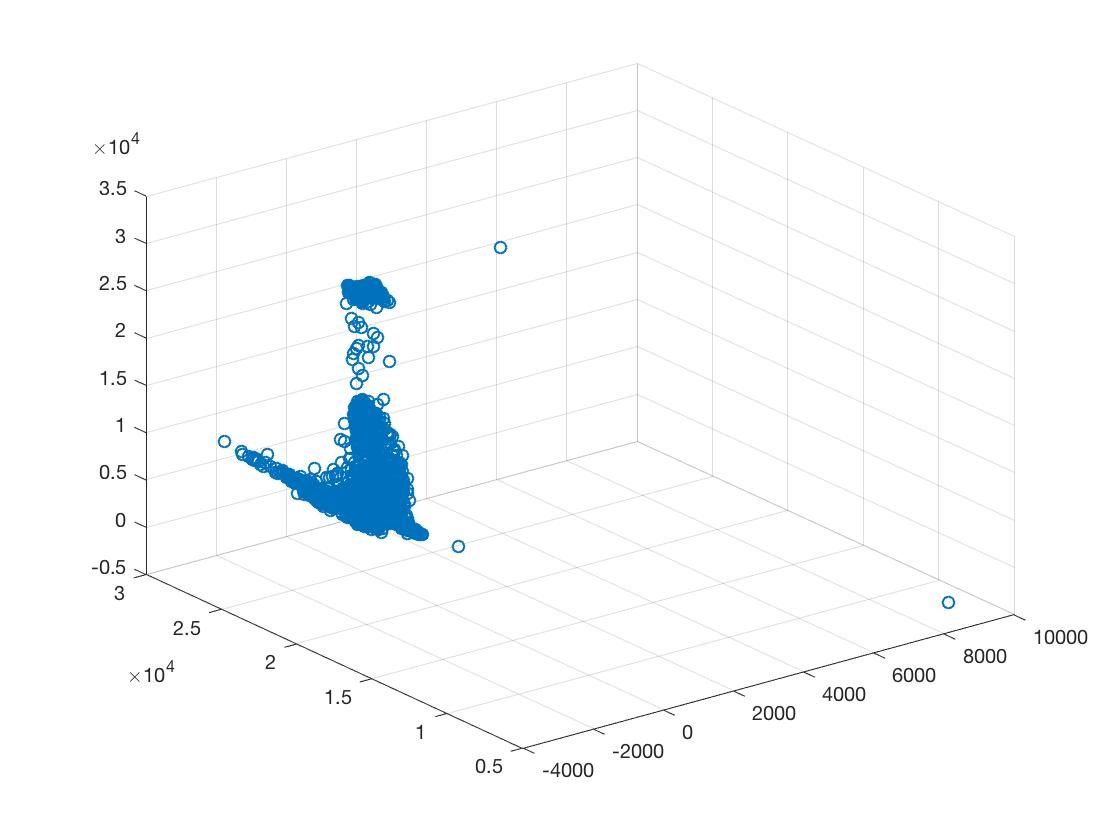
\includegraphics[width=4cm, height=4cm]{pic/pca3d}}
\end{figure}

The 3d plot of the first three Laplacian eigenvectors shows that the pixel points can be easily categorized into 3 clusters by kmeans. This 3d space is subspace of graph eigenspace. (knn=15 sigma = 50000)

\begin{figure}[h]
  \centering
  \subfloat[ Eigenspace ]{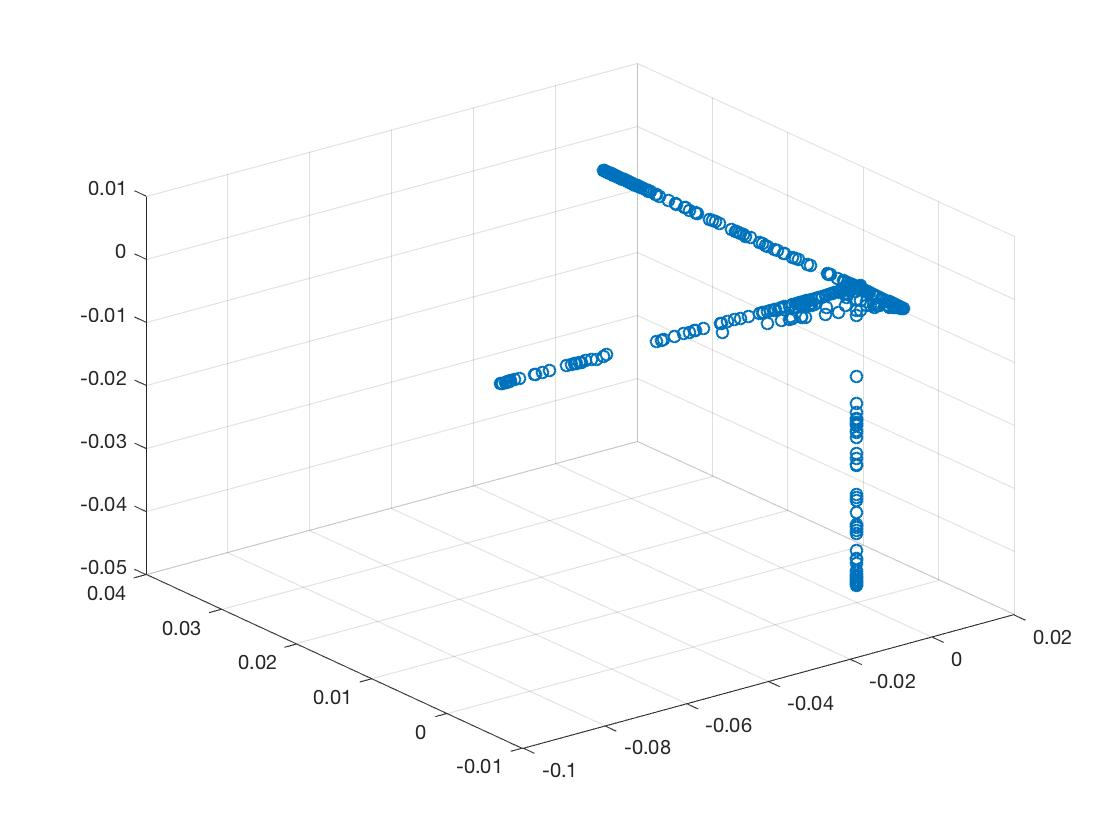
\includegraphics[width=4cm, height=4cm]{pic/sc3d}}
\end{figure}

\subsection*{Attachment : Codes}
\subsubsection{Question3a:spectral clustering}
\begin{lstlisting}
clear all;
load('SalinasA_corrected.mat');
close all;

data1D = reshape(salinasA_corrected,[],204);


%% Sparse construction
sigma=50;

W_sparse=sparse(size(data1D,1),size(data1D,1));
Knn=15;
NN=zeros(Knn,size(data1D,1));

for i=1:size(data1D,1)
    NN(:,i)=knnsearch(data1D,data1D(i,:),'k',Knn);
    for j=1:Knn
       W_sparse(i,NN(j,i))=exp(-norm(data1D(i,:)-data1D(NN(j,i),:)).^2/sigma^2);
%       W_sparse(i,NN(j,i))=(norm(data1D(i,:)-data1D(NN(j,i),:)));
    end
end

D_sparse=diag(sum(W_sparse,2));

L_sparse=eye(size(W_sparse))-D_sparse^(-1)*W_sparse;

[EigVecsSparse,EigValsSparse]=eigs(L_sparse,10,'sr');
EigValsSparse=diag(EigValsSparse);

close all;

%% Display Ng, Jordan, Weiss clustering

Labels=kmeans(EigVecsSparse(:,1:6),6,'Replicates',100);

im = image(reshape(Labels,83,86),'CDataMapping','scaled');
colorbar

%% sigma vs egienvalues
plot(fliplr(EigValsSparse'))

\end{lstlisting}

\subsubsection{PCA}
\begin{lstlisting}

clear all;
load('SalinasA_corrected.mat');
close all;

data1D = reshape(salinasA_corrected,[],204);
pcaM=pca(data1D);
projData=data1D*pcaM;

pca1=reshape(projData(:,1),83,86);

pca1=reshape(projData(:,1),83,86);
image(pca1,'CDataMapping','scaled');

pca2=reshape(projData(:,2),83,86);
image(pca2,'CDataMapping','scaled');

pca3=reshape(projData(:,3),83,86);
image(pca3,'CDataMapping','scaled');
\end{lstlisting}

\end{document}
